% =====================================================================
% AIM 3 EDITS FOR OVERLEAF -- paste-ready snippets (from export 7 base)
% =====================================================================

% ---------------------------------------------------------------------
% 1) INNOVATION, subsubsection "Predictive capability of Digital Twins":
%    replace the red line "To do: Add some previous works related to G&R"
%    with this paragraph (it ends right before the existing bold
%    "For our current cohort..." sentence).
% ---------------------------------------------------------------------
The predictive reach of DTs has so far ended at the heartbeat time scale. Models of cardiac \gls*{gr}, which unfolds over months, have been dominated by kinematic growth theory\cite{rodriguez94}: prescribing where and how much the ventricle grows, these models reproduce the shape changes of hypertrophy, dilation, and infarction\cite{goktepe10,costabal19,saez15}, but they cannot answer whether a given ventricle will grow, because the growth is imposed rather than predicted. The constrained mixture theory\cite{humphrey02a} instead lets growth emerge from the turnover of myocytes and collagen chasing a homeostatic mechanical set-point, and its homogenized formulation\cite{cyron16,braeu16} made this mechanistic description tractable at organ scale. Building on it, we developed the first homogenized constrained mixture model of cardiac \gls*{gr}\cite{gebauer23} and made it efficient enough for months-long, patient-specific simulation\cite{gebauer24}. Applying it to forecast whether a recruited borderline ventricle will reach a size that can sustain a \gls*{biv} circulation is, to our knowledge, the first mechanistic prediction of ventricular recruitment adequacy. Its actionable output is the identification, before any surgery, of the children whose ventricles will not grow enough.

% ---------------------------------------------------------------------
% 2) PRELIMINARY DATA: insert this block at the end of the subsection,
%    BEFORE the sentence "Based on our preliminary trials, we will
%    describe how our current research aims will be pursued."
%    Also DELETE the same wrapfigure (label fig_cardiac_gr) from the
%    Aim 3 subsection, where it currently lives.
% ---------------------------------------------------------------------
\begin{wrapfigure}{r}{0.4\textwidth}
    \centering
    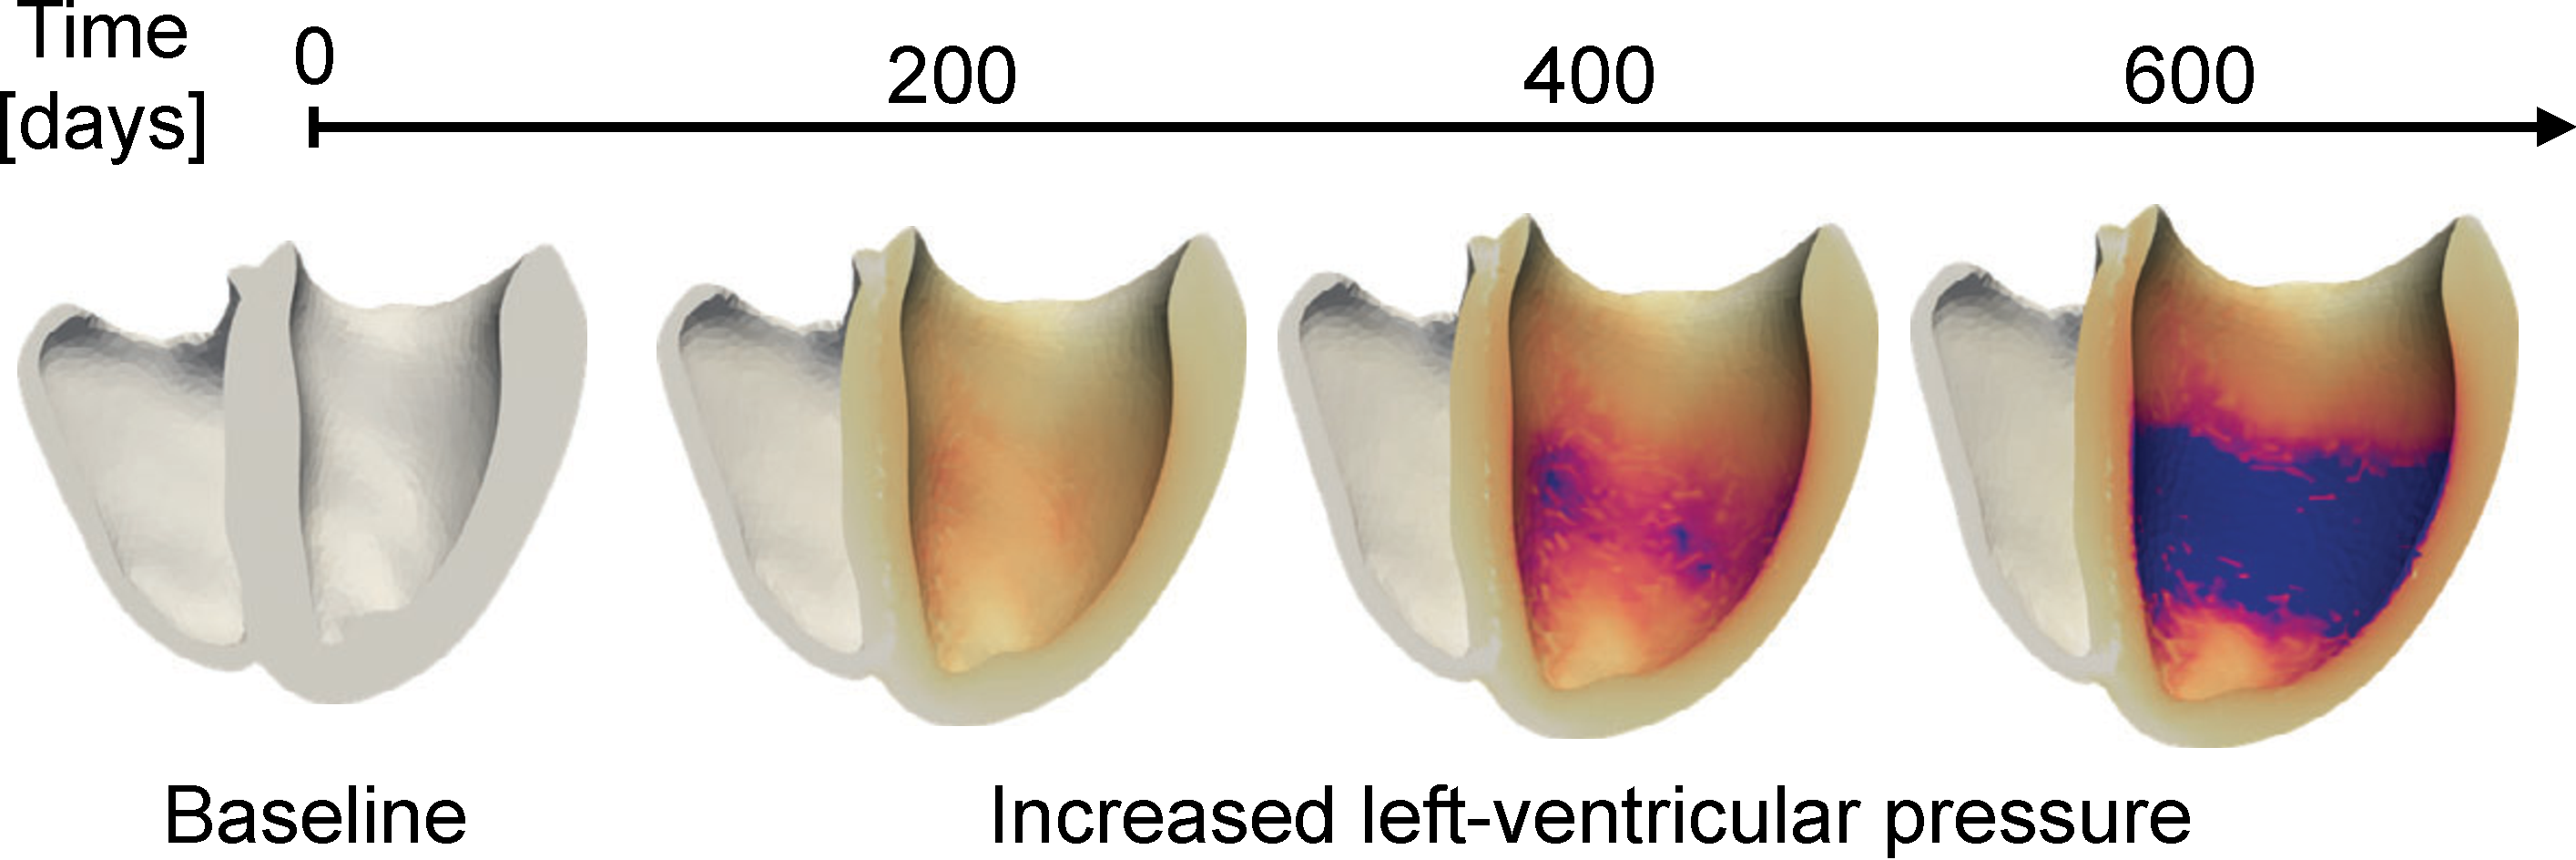
\includegraphics[width=0.4\textwidth]{figures/figures_gr_page1.pdf}
    \caption{\textbf{Predicted long-term cardiac \gls*{gr} in left-ventricular pressure overload.} Ventricles are colored by local mass increase from white (0\%) to purple (100\%). Adapted from Gebauer et al.\cite{gebauer24}}
    \label{fig_cardiac_gr}
    \vspace{-6pt}
\end{wrapfigure}
\textbf{Long-term growth and remodeling.} For the long-term counterpart of these short-term predictions, we developed and validated the first \gls*{hcmm} of cardiac \gls*{gr}\cite{gebauer23}, in which organ-scale growth emerges from the deposition and degradation of myocyte and collagen constituents driven by the deviation of their stress from a homeostatic set-point. From a single set of equations, the model reproduces both stable growth that returns to homeostasis and unstable, runaway dilation, and it captures the reversal of growth once the load is relieved, reproducing reference constrained-mixture behavior at a fraction of the computational cost\cite{gebauer23}. Adaptive integration of the history variables makes patient-specific simulation over months of physiological time practical\cite{gebauer24}, illustrated by the predicted \gls*{gr} of a left ventricle under pressure overload in Figure~\ref{fig_cardiac_gr}. Aim 3 initializes this model from each child's pre-recruitment \gls*{dt}.

% ---------------------------------------------------------------------
% 3) AIM 3: replace the whole "Feasibility and rigor of prior research."
%    paragraph with this slimmed version (details now live in
%    Innovation and Preliminary Data).
% ---------------------------------------------------------------------
\textbf{Feasibility and rigor of prior research.} The choice of model class is central to feasibility. Kinematic growth models\cite{rodriguez94,goktepe10} prescribe the direction and extent of growth and therefore cannot decide whether a borderline ventricle will grow enough. Predicting growth requires a mechanistic model in which growth emerges from constituent turnover\cite{humphrey02a,cyron16,braeu16}. Both capabilities this aim requires are in hand and validated, as summarized in the Preliminary Data (Figure~\ref{fig_cardiac_gr}): our \gls*{hcmm} of cardiac \gls*{gr} predicts organ-scale ventricular change from constituent-level turnover\cite{gebauer23}, and its adaptive integration makes months-long, patient-specific simulation efficient\cite{gebauer24}. The growth model builds on the reduced-geometry heart model and PhysioBlocks implementation of Aims 1 and 2\cite{caruel13}, so it shares the \gls*{dt} geometry, kinematics, and constitutive laws. Because Aim 3 operates on \glspl*{dt} constructed offline from stored \gls*{icmr} data, it is independent of the real-time pipeline of Aim 1. As an early go/no-go, in Year 1 we will reproduce a single retrospective paired case (pre- and post-recruitment \gls*{icmr}) end to end before scaling to the cohort.

% ---------------------------------------------------------------------
% 4) BIB FIXES to replicate in Overleaf:
%    a) references.bib: fix the Tuma accent in jarolimova_AJP2026:
%       T{\uu}ma  ->  T{\r u}ma   (\uu is not a LaTeX macro; this
%       breaks the PDF build once the entry is cited)
%    b) grant_application.tex: two cites spell the key "gall20" while the
%       bib entry is "legall20" -- change both to legall20.
%    c) references.bib: add this entry (cited in Aim 1, in neither bib):
@article{skardova_Heliyon2026,
  title={Combining machine learning and mathematical modeling in inverse problems: {A}pplication to estimation of {T}1 relaxation time from cardiac magnetic resonance imaging data},
  author={{\v{S}}kardov{\'a}, Kate{\v{r}}ina and Galabov, Radek and Frickov{\'a}, Kate{\v{r}}ina and Pevn{\'y}, Tom{\'a}{\v{s}} and Tint{\v{e}}ra, Jaroslav and Oberhuber, Tom{\'a}{\v{s}} and \textbf{Chabiniok R}},
  journal={Heliyon},
  volume={12},
  number={10},
  year={2026},
  publisher={Elsevier}
}
